%%%%%%%%%%%%%%%%%%%%%%%%%%%%%%%%%%%%%
%                                   %
% Compile with XeLaTeX and biber    %
%                                   %
% Questions or comments:            %
%                                   %
% joshua dot mcneill at uga dot edu %
%                                   %
%%%%%%%%%%%%%%%%%%%%%%%%%%%%%%%%%%%%%

\documentclass{beamer}
  % Read in standard preamble (cosmetic stuff)
  %%%%%%%%%%%%%%%%%%%%%%%%%%%%%%%%%%%%%%%%%%%%%%%%%%%%%%%%%%%%%%%%
% This is a standard preamble used in for all slide documents. %
% It basically contains cosmetic settings.                     %
%                                                              %
% Joshua McNeill                                               %
% joshua dot mcneill at uga dot edu                            %
%%%%%%%%%%%%%%%%%%%%%%%%%%%%%%%%%%%%%%%%%%%%%%%%%%%%%%%%%%%%%%%%

% Beamer settings
% \usetheme{Berkeley}
\usetheme{CambridgeUS}
% \usecolortheme{dove}
% \usecolortheme{rose}
\usecolortheme{seagull}
\usefonttheme{professionalfonts}
\usefonttheme{serif}
\setbeamertemplate{bibliography item}{}

% Packages and settings
\usepackage{fontspec}
  \setmainfont{Charis SIL}
\usepackage{hyperref}
  \hypersetup{colorlinks=true,
              allcolors=blue}
\usepackage{graphicx}
  \graphicspath{{../../figures/}}
\usepackage[normalem]{ulem}
\usepackage{enumerate}

% Document information
\author{M. McNeill}
\title[FREN2001]{Français 2001}
\institute{\url{joshua.mcneill@uga.edu}}
\date{}

%% Custom commands
% Lexical items
\newcommand{\lexi}[1]{\textit{#1}}
% Gloss
\newcommand{\gloss}[1]{`#1'}
\newcommand{\tinygloss}[1]{{\tiny`#1'}}
% Orthographic representations
\newcommand{\orth}[1]{$\langle$#1$\rangle$}
% Utterances (pragmatics)
\newcommand{\uttr}[1]{`#1'}
% Sentences (pragmatics)
\newcommand{\sent}[1]{\textit{#1}}
% Base dir for definitions
\newcommand{\defs}{../definitions}


  % Packages and settings

  % Document information
  \subtitle[Meubles et objets indirects]{Décrivant les meubles et les grands nombres}

\begin{document}
  % Read in the standard intro slides (title page and table of contents)
  \begin{frame}
    \titlepage
    \tiny{Office: % Basically a variable for office hours location
Gilbert 121\\
          Office hours: % Basically a variable for office hours
 lundi, mercredi, vendredi 10:10--11:10
}
  \end{frame}

  \begin{frame}{Dates et nombres}
    \begin{columns}
      \scriptsize
      \column{0.5\textwidth}
        Répondre aux questions suivantes:
        \begin{enumerate}
          \item Quelle est la date? \underline{\uncover<2->{Le 20 janvier 2023}}
          \item<3-> En quelle année les États-Unis sont-ils entrés dans la Seconde Guerre mondiale? \underline{\uncover<4->{1941}}
          \item<5-> En quelle année a-t-on écrit la Déclaration d'indépendance? \underline{\uncover<6->{1776}}
          \item<7-> Quel a été le revenu médian des ménages \gloss{households} aux États-Unis en 2021? \underline{\uncover<8->{70~784 \$}}
          \item<9-> Quel est le coût moyen \gloss{average} des maisons à Athens? \underline{\uncover<10->{312~376 \$}}
          \item<11-> Quel est le salaire annuel de Kirby Smart? \underline{\uncover<12->{7~200~000 \$}}
          \item<13-> Combien coûte ce canapé? \underline{\uncover<14->{51~980 \$}}
          \item<15-> Combien coûte cette table basse? \underline{\uncover<16->{10~000 \$}}
        \end{enumerate}
      \column{0.5\textwidth}
        \begin{minipage}[t][0.6\textheight]{\linewidth}
          \begin{center}
            \only<3-4>{
              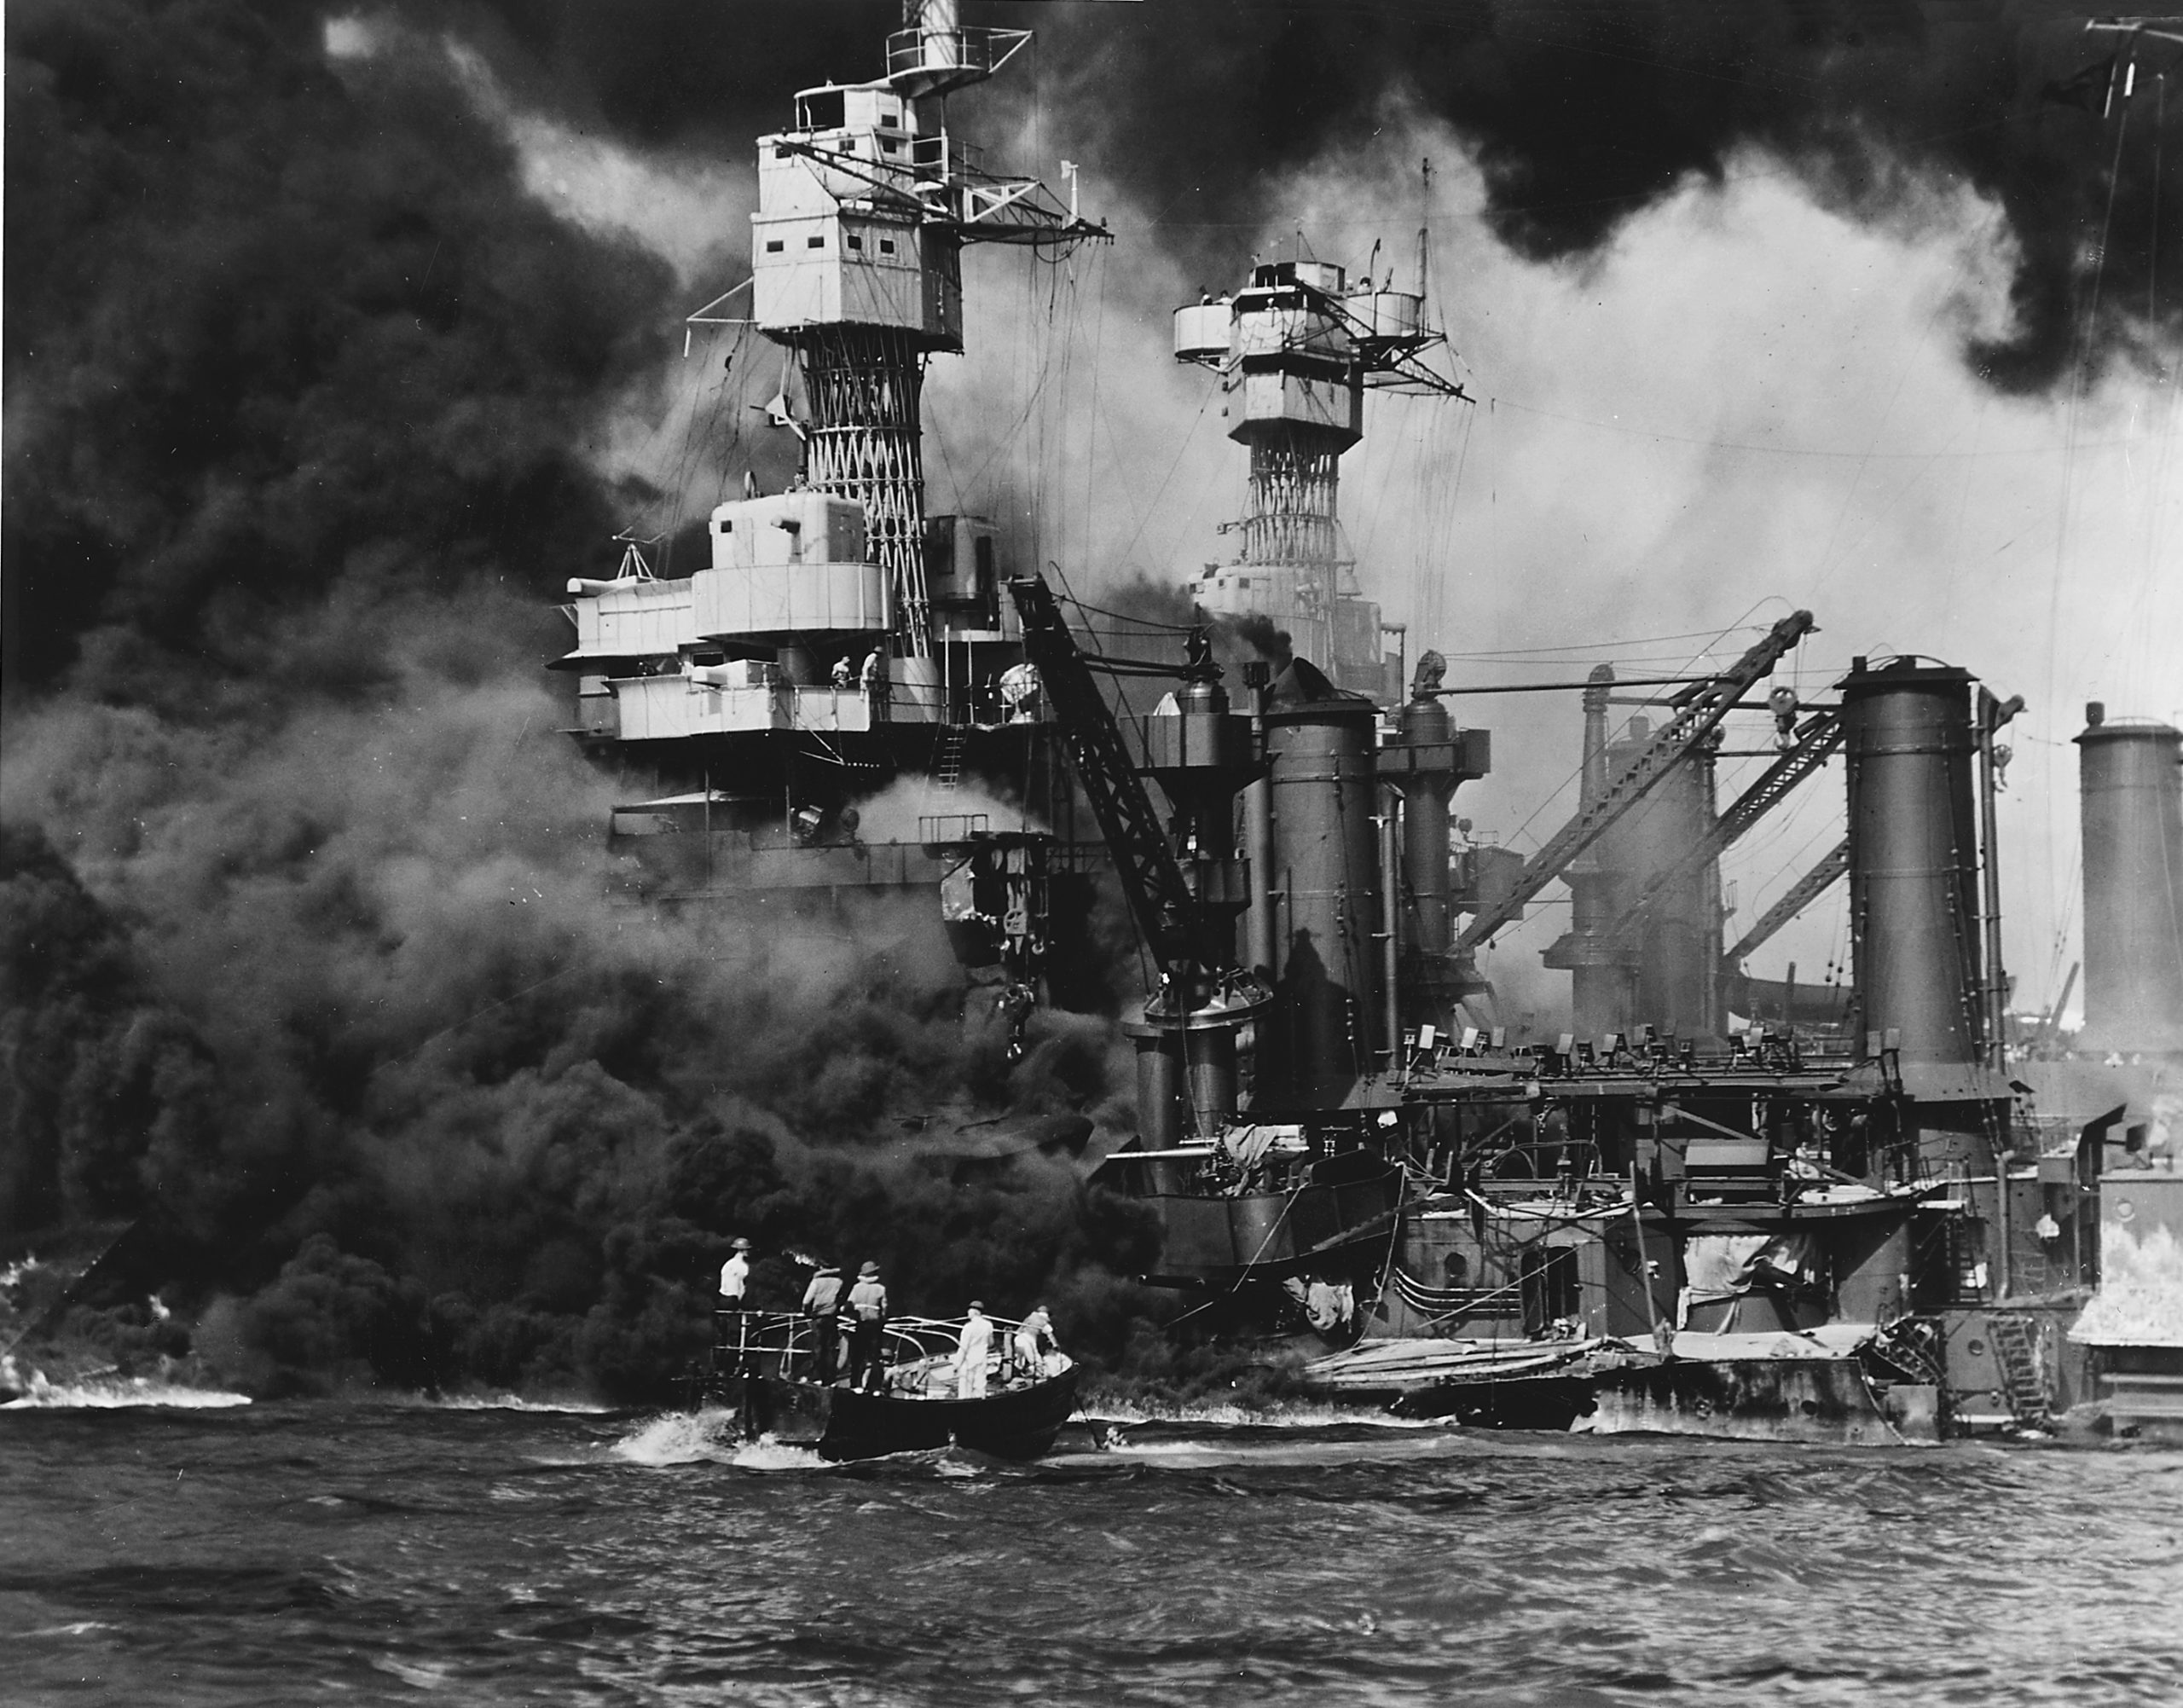
\includegraphics[scale=0.28]{wwii.jpg} \\
              Pearl Harbor
            }
            \only<5-6>{
              \includegraphics[scale=0.08]{déclaration.jpg}
            }
            \only<7-10>{
              \includegraphics[scale=0.4]{revenu_médian.jpg}
            }
            \only<11-12>{
              
\includegraphics[scale=0.23]{kirby_smart.jpg}
            }
            \only<13-14>{
              \includegraphics[scale=0.3]{canapé.jpg}
            }
            \only<15-16>{
              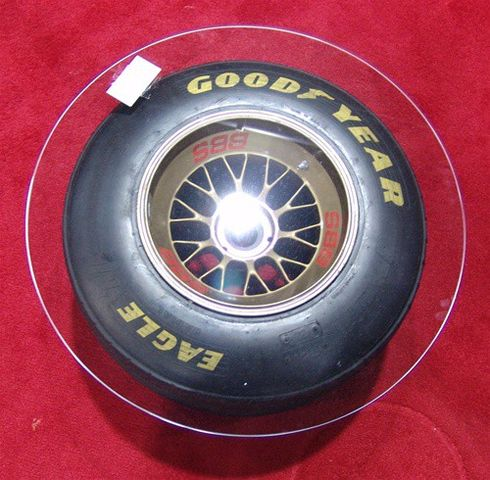
\includegraphics[scale=0.3]{table_basse.jpg} \\
              \uncover<16->{Un pneu \gloss{tire} utilisé par Michael Schumacher}
            }
          \end{center}
        \end{minipage}
    \end{columns}
  \end{frame}

  \begin{frame}{}
    \begin{center}
      \Large Quiz
    \end{center}
  \end{frame}

  \begin{frame}{Décrire une salle}
    Avec un/e partenaire, décris une salle pour que ton partenaire dessine la salle.
    {\scriptsize
    \begin{description}
      \item[\textbf{Modèle:}]
      \item[E1:] La salle est ma chambre. Il y a une fenêtre pratique à côté de mon lit abîmé. Une chaise se trouve près de la porte bleue et l'autre chaise entre le lit et la fenêtre. \textit{etc}...
      \item[E2:]
    \end{description}
    \begin{center}
      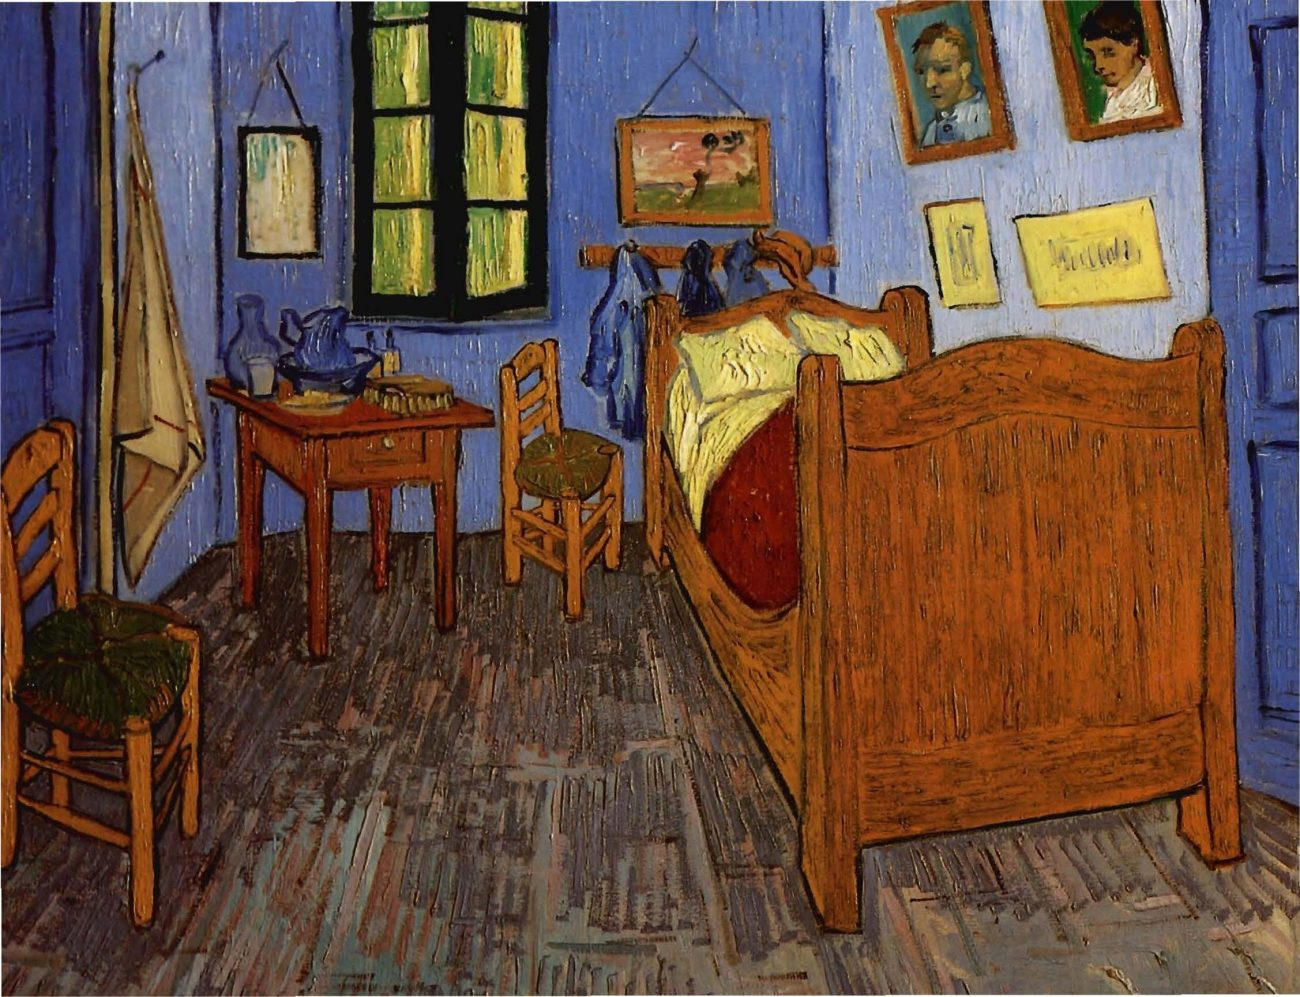
\includegraphics[scale=0.125]{van_gogh.jpg} \\
      La Chambre de Van Gogh à Arles (1889)
    \end{center}
    }
  \end{frame}

  \begin{frame}{}
    \begin{center}
      \Large Questions?
    \end{center}
  \end{frame}
\end{document}
